\documentclass[11pt]{article}
\usepackage[margin=0.78in]{geometry}
\usepackage{amsmath,amssymb,booktabs,graphicx,microtype,xcolor}
\usepackage[hidelinks]{hyperref}
\usepackage[font=small,labelfont=bf]{caption}
\usepackage{enumitem}
\definecolor{atlasblue}{HTML}{176B87}
\hypersetup{colorlinks=true,linkcolor=atlasblue,citecolor=atlasblue,urlcolor=atlasblue}
\setlength{\parindent}{0pt}
\setlength{\parskip}{5pt}
\setlist[itemize]{leftmargin=1.3em,itemsep=2pt,topsep=3pt}
\newcommand{\fedd}{f_{\mathrm{Edd}}}
\newcommand{\mbh}{M_{\mathrm{BH}}}
\newcommand{\mseed}{M_{\mathrm{seed}}}

\title{\textbf{Constraining Black Hole Growth in the JWST Era}}
\author{Nicole Jiang}
\date{Draft: 7 September 2026}

\begin{document}
\maketitle

\begin{abstract}
\textbf{Aims.} We assess which JWST-identified accreting black holes and
candidates at $z\geq4$ place meaningful constraints on early growth histories,
and how these constraints depend on seed formation, radiative efficiency,
and reported mass uncertainty.

\textbf{Methods.} We compile a provenance-aware catalogue containing 350
literature measurements across 32 source families, represented by 338
object records in 337 host systems pending final identity reconciliation.
Our primary comparison uses 227 objects with comparable mass methods and
accepted evidence classifications; an exploratory analysis includes all 237
objects with eligible numerical masses. The other 101 remain explicit
no-inference records. We propagate published asymmetric mass
errors using 10,000 deterministic Monte Carlo draws and preserve mass-method
systematics as separate envelopes. We compare fixed seed, formation-redshift,
and efficiency scenarios using a reproducible catalogue workflow.

\textbf{Results.} Under the reference assumptions $z_{\rm seed}=30$,
$\epsilon=0.1$, no merger boost, and a $10^2\,M_\odot$ seed, 12 primary-sample
objects require a lifetime-average $\fedd>1$ at their point estimates. Eight
remain above unity at the 16th percentile, and six have
$P(\fedd>1)\geq0.95$. The corresponding exploratory counts are 14, ten, and eight.
UNCOVER-20466 has the highest required average rate, with median
$\fedd=1.453$ and a 16th--84th percentile interval of 1.354--1.549.
Increasing the seed mass to $10^3\,M_\odot$ reduces the primary count above
unity to four; delaying seeding to $z_{\rm seed}=20$ increases it to 22.
At the ideal non-spinning thin-disk efficiency $\epsilon=0.05719$, no point
estimate in either sample requires $\fedd>1$ under otherwise unchanged assumptions. The
inferred growth requirements are therefore conditional on the adopted model;
heterogeneous selection functions and mass estimators preclude interpreting
global rankings as demographic measurements.

\smallskip
\noindent\textbf{Key words.} black hole physics -- accretion, accretion disks --
galaxies: active -- galaxies: high-redshift -- quasars: supermassive black holes
\end{abstract}

\section{Introduction}

The discovery of massive black holes in the early Universe raises a fundamental
question: what growth histories could have assembled them within the available
cosmic time? The strength of this constraint depends on both the observed
black-hole mass and redshift, as well as assumptions about seed formation,
radiative efficiency, and the duration of active accretion. An apparently
demanding object under one set of assumptions may therefore be compatible with
less extreme growth under another.

Here, we use a literature-based catalogue of JWST-identified high-redshift
accreting black holes and candidates to ask which objects meaningfully constrain
early growth histories. The atlas covers $z\geq4$, extending from the first
billion years to a cosmic age of approximately 1.54 Gyr at its lower-redshift
boundary. We calculate the average accretion rates required across a range of
seed and growth assumptions, incorporating reported mass uncertainties and
distinguishing measurements with different evidential and methodological
limitations. Source-native measurements, identity links, and mass provenance
are retained to support comparison across heterogeneous literature samples.

Our aim is to identify which growth requirements remain demanding across
plausible scenarios, which depend primarily on uncertain assumptions, and where
improved observations would most strengthen the constraints. This approach
treats the catalogue as a means of testing possible growth histories, rather
than assuming that every high-redshift black hole presents the same assembly
problem. The constraints apply to individual objects under stated assumptions;
we do not estimate a pooled mass function, occurrence rate, or formation-channel
fraction.

Analytic seed-growth comparisons already establish the trade-off between seed
mass and sustained accretion. For example, Dayal \cite{dayal2024} considered
light and heavy seeds at $z_{\rm seed}=25$ and explored a primordial-seeding
interpretation. Here we use this established growth framework to assess how
object-level constraints change when published masses, measurement methods,
and growth assumptions are treated consistently across a larger evidence atlas.
The contribution is a traceable comparison of which constraints persist under
reported mass uncertainty and which disappear when assumptions change; we do
not infer a primordial abundance or introduce a new growth mechanism.
The source-family inventory is given in Appendix~\ref{app:sources}.

\subsection{Theoretical framework}
\label{sec:theory}

The growth constraints follow from the relation between accretion luminosity,
retained mass, and available cosmic time. For electron-scattering opacity in
ionized hydrogen, the Eddington luminosity and luminosity-based Eddington ratio
are
\begin{equation}
L_{\rm Edd}=\frac{4\pi G\mbh m_p c}{\sigma_T},\qquad
\fedd=\frac{L_{\rm bol}}{L_{\rm Edd}},\qquad
t_{\rm Edd}=\frac{\mbh c^2}{L_{\rm Edd}}
=\frac{c\sigma_T}{4\pi Gm_p}\simeq0.45\ {\rm Gyr}.
\label{eq:eddington}
\end{equation}
Here $G$, $c$, $m_p$, and $\sigma_T$ denote the gravitational constant,
speed of light, proton mass, and Thomson cross section. With radiative
efficiency $0<\epsilon<1$ and rest-mass inflow rate $\dot M_{\rm in}$,
\begin{equation}
L_{\rm bol}=\epsilon\dot M_{\rm in}c^2,\qquad
\dot\mbh=(1-\epsilon)\dot M_{\rm in}
=\frac{1-\epsilon}{\epsilon}\frac{\fedd}{t_{\rm Edd}}\mbh.
\label{eq:massgrowth}
\end{equation}
The inflow rate is defined at the radiating flow; additional mass loss before
that point is not modelled. At fixed efficiency, define
\begin{equation}
\Delta t=t(z_{\rm obs})-t(z_{\rm seed})>0,\qquad
\overline{\fedd}=\frac{1}{\Delta t}
\int_{t(z_{\rm seed})}^{t(z_{\rm obs})}\fedd(t)\,dt.
\label{eq:average}
\end{equation}
The analytic growth relation adopted by Dayal \cite{dayal2024} then becomes
\begin{equation}
\mbh(t_{\rm obs})=B_{\rm merge}\mseed
\exp\!\left[\frac{1-\epsilon}{\epsilon}
\frac{\overline{\fedd}\,\Delta t}{t_{\rm Edd}}\right],\qquad
t_{\rm efold}=\frac{\epsilon}{1-\epsilon}
\frac{t_{\rm Edd}}{\fedd}.
\label{eq:growth}
\end{equation}
The e-folding time assumes constant positive $\fedd$; it is 0.05 Gyr at
$\epsilon=0.1$ and $\fedd=1$. The dimensionless $B_{\rm merge}$ represents an
effective multiplicative merger boost, not a resolved merger history.

Cosmic ages use the flat matter-plus-Lambda relation
\begin{equation}
t(z)=\frac{2}{3H_0\sqrt{\Omega_\Lambda}}
\operatorname{asinh}\!\left[\sqrt{\frac{\Omega_\Lambda}{\Omega_m}}
(1+z)^{-3/2}\right],
\label{eq:cosmictime}
\end{equation}
with $H_0=67.3\,{\rm km\,s^{-1}\,Mpc^{-1}}$, $\Omega_m=0.315$, and
$\Omega_\Lambda=0.685$. The Hubble constant is converted to inverse time;
ages and growth intervals are in Gyr. Radiation is neglected. In particular,
the supplementary $z_{\rm seed}=3400$ comparison extrapolates this age relation
and is not a radiation-era seed-formation calculation.

Two inversions provide the principal growth diagnostics:
\begin{align}
\overline{\fedd}_{\rm req}
&=\max\!\left[0,\frac{\epsilon}{1-\epsilon}
\frac{t_{\rm Edd}}{\Delta t}
\ln\!\left(\frac{\mbh}{B_{\rm merge}\mseed}\right)\right],
\label{eq:required-rate}\\
\log_{10}\!\left(\frac{M_{\rm seed,req}}{M_\odot}\right)
&=\log_{10}\!\left(\frac{\mbh}{M_\odot}\right)-\log_{10}B_{\rm merge}
-\frac{1-\epsilon}{\epsilon}
\frac{\overline{\fedd}\,\Delta t}{t_{\rm Edd}\ln 10}.
\label{eq:required-seed}
\end{align}
In Eq.~\ref{eq:required-seed}, $M_{\rm seed,req}$ denotes the required seed
mass. The zero floor in Eq.~\ref{eq:required-rate} follows the implementation:
if the boosted seed already exceeds the observed mass, no positive accretion
is required, but this does not make that fixed history an exact mass match.

For a two-state history with the same efficiency in both states,
\begin{equation}
\overline{\fedd}=D f_{\rm burst}+(1-D)f_{\rm quiet},\qquad
D_{\rm req}=\frac{\overline{\fedd}_{\rm req}-f_{\rm quiet}}
{f_{\rm burst}-f_{\rm quiet}}.
\label{eq:dutycycle}
\end{equation}
Here $D$ is the active-state time fraction, $f_{\rm burst}>f_{\rm quiet}\geq0$,
and the diagnostic requires $\overline{\fedd}_{\rm req}\geq f_{\rm quiet}$.
Values $D_{\rm req}>1$ identify an infeasible specified two-state history and
are retained. An average growth requirement is not an instantaneous Eddington
ratio or a uniquely measured duty cycle.

For the illustrative spin-dependent maps, the ideal Kerr thin-disk efficiency
is the ISCO binding efficiency \cite{bardeen1972}:
\begin{align}
\epsilon_a&=1-\sqrt{1-\frac{2}{3r_{\rm ISCO}}},\\
r_{\rm ISCO}&=3+Z_2-\operatorname{sgn}(a)
\sqrt{(3-Z_1)(3+Z_1+2Z_2)},\\
Z_1&=1+(1-a^2)^{1/3}\big[(1+a)^{1/3}+(1-a)^{1/3}\big],\qquad
Z_2=\sqrt{3a^2+Z_1^2}.
\label{eq:spin}
\end{align}
The dimensionless spin is $a=cJ/(G\mbh^2)$, where $J$ is the signed angular
momentum relative to the disk, and $r_{\rm ISCO}$ is in units of $G\mbh/c^2$.
The ideal efficiencies at $a=-1,0,+1$ are approximately 0.038, 0.057, and
0.423, respectively, neglecting photon capture and stress at the ISCO.
Above unity, the maps adopt a phenomenological luminosity ansatz,
\begin{equation}
\fedd=1+\ln\dot m,\qquad
\dot m=\frac{\dot M_{\rm in}}{L_{\rm Edd}/(\epsilon_a c^2)},\qquad
\epsilon_{\rm eff}=\begin{cases}
\epsilon_a,&\fedd\leq1,\\
\epsilon_a\fedd\exp(1-\fedd),&\fedd>1.
\end{cases}
\label{eq:effective-efficiency}
\end{equation}
The logarithmic luminosity ansatz applies only on the super-Eddington branch.
This is an illustrative parameter-scan prescription, not a relativistic
slim-disk or spin-evolution calculation. If efficiency varies with time, the
integrated growth depends on $\int [(1-\epsilon(t))/\epsilon(t)]\fedd(t)\,dt$;
it cannot in general be represented by separately averaged efficiency and rate.

\section{Catalogue construction}

\subsection{Scope and versioning}

The catalogue uses scientific dataset versions rather than software releases.
v1 is the original 23-object JADES broad-line catalogue. v2 expands the same
mass-comparable analysis to 211 JWST broad-line objects. v3 retains all v2
objects and adds heterogeneous JWST-identified evidence classes. A source enters
only one admission version; an internally heterogeneous source is assigned in
full to v3. The fixed scope requires $z\geq4$ and identification or candidate
classification from JWST data. Objects merely followed up by JWST after a
non-JWST discovery are outside the admission rule.

Source-family and measurement membership is frozen at the review cutoff of
3 September 2026; corrections to admitted measurements apply across affected
versions, while new measurements require a declared subsequent version.

The v3 catalogue has 350 measurement rows, 338 provisional object records, and
337 provisional host records. All object-level sample sizes below inherit the
three open identity groups described in Section~\ref{sec:limits}. It contains 247 broad-line AGN, 49 narrow-line candidates, 30
photometric candidates, ten high-ionization candidates, and two X-ray
candidates. Preferred object-level evidence comprises 214 secure, 41 probable,
82 candidate, and one disputed classification. These labels describe the source
papers' evidence and do not place all classes on a single purity scale.

\subsection{Provenance, extraction, and identity}

Each measurement carries stable measurement, physical-object, and host-system
identifiers. Source-native values, adopted standardized values, uncertainty
semantics, table locations, URLs, DOI or archive versions, archive SHA-256
hashes where available, extraction dates, and caveat tags are retained. The
manual-extraction audit covers 26 hash-pinned extraction artifacts, while the
provenance registry contains 38 records covering all 32 admitted source
families. Independent checks cover all 244 numerical masses and both error fields. Auxiliary coordinate and contextual sources are attributed separately
to the THRILS catalogue \cite{hutchison2025}, the UHZ1 spectroscopy paper
\cite{goulding2023}, and the versioned JADES DR3 GOODS-S prism catalogue.

Identity resolution preserves every admitted measurement while selecting one
preferred row for object-level inference. Alternate measurements are never
silently averaged. The final completion illustrates this policy: 15 NEXUS
NIRCam/WFSS measurements \cite{zhuang2025}, 13 COSMOS-3D NIRCam-grism
measurements \cite{lin2025}, and GHZ4/GHZ7 \cite{napolitano2024} add 30
measurements but 29 object records. NEXUS source NX10835 lies 0.066 arcsec from
an existing Mascia identifier at consistent redshift, so the new mass-bearing
measurement becomes preferred for the same object.

The Scholtz et al. source audit provides another cardinality check. The paper
reports 42 objects, whereas its source-native table contains 41 rows. Exactly 21
table rows satisfy $z\geq4$; all are admitted. One is identity-linked to a
broad-line object, yielding 20 distinct narrow-line candidates from that source.
JADES-NS-GS00099671 is retained with its published host and bolometric
observables but without an invented black-hole mass.

\subsection{Mass comparability and analysis subsets}

A measurement enters numerical growth analysis only when the source publishes a
canonical numeric black-hole mass compatible with the declared comparison
policy. Conditional masses inferred by assuming an Eddington ratio, indirect
model ranges, and upper limits remain contextual observables. This produces 244
eligible measurements and 237 eligible preferred objects. Of those objects, 236
use Balmer-line single-epoch virial masses and one uses a UV single-epoch virial
mass. Their redshifts span 4.000--10.603 with median 5.110; standardized
$\log_{10}(\mbh/M_\odot)$ spans 5.51--9.31 with median 7.18. The 101 objects
without an eligible mass remain visible throughout the catalogue and atlas.
The stricter primary subset has 234 measurements and 227 preferred objects:
it excludes candidate or disputed evidence, conditional mass interpretations,
and methods not flagged as primary-comparable. Numerical eligibility alone
therefore does not imply membership in the primary comparison subset.

\begin{table}[ht]
\centering
\caption{v3 scale and analysis subsets.}
\begin{tabular}{@{}lr@{}}
\toprule
Product or subset & Rows or objects \\
\midrule
Measurements / provisional objects / hosts & 350 / 338 / 337 \\
Source-local observables & 810 \\
Growth-eligible measurements / objects & 244 / 237 \\
Primary-analysis measurements / objects & 234 / 227 \\
Catalogue-only object records & 101 \\
Alternate-measurement sensitivity pairs & 7 \\
Source-family caveat rows & 32 \\
Per-object parameter-map panels & 676 \\
\bottomrule
\end{tabular}
\label{tab:scale}
\end{table}

\begin{figure}[p]
\centering
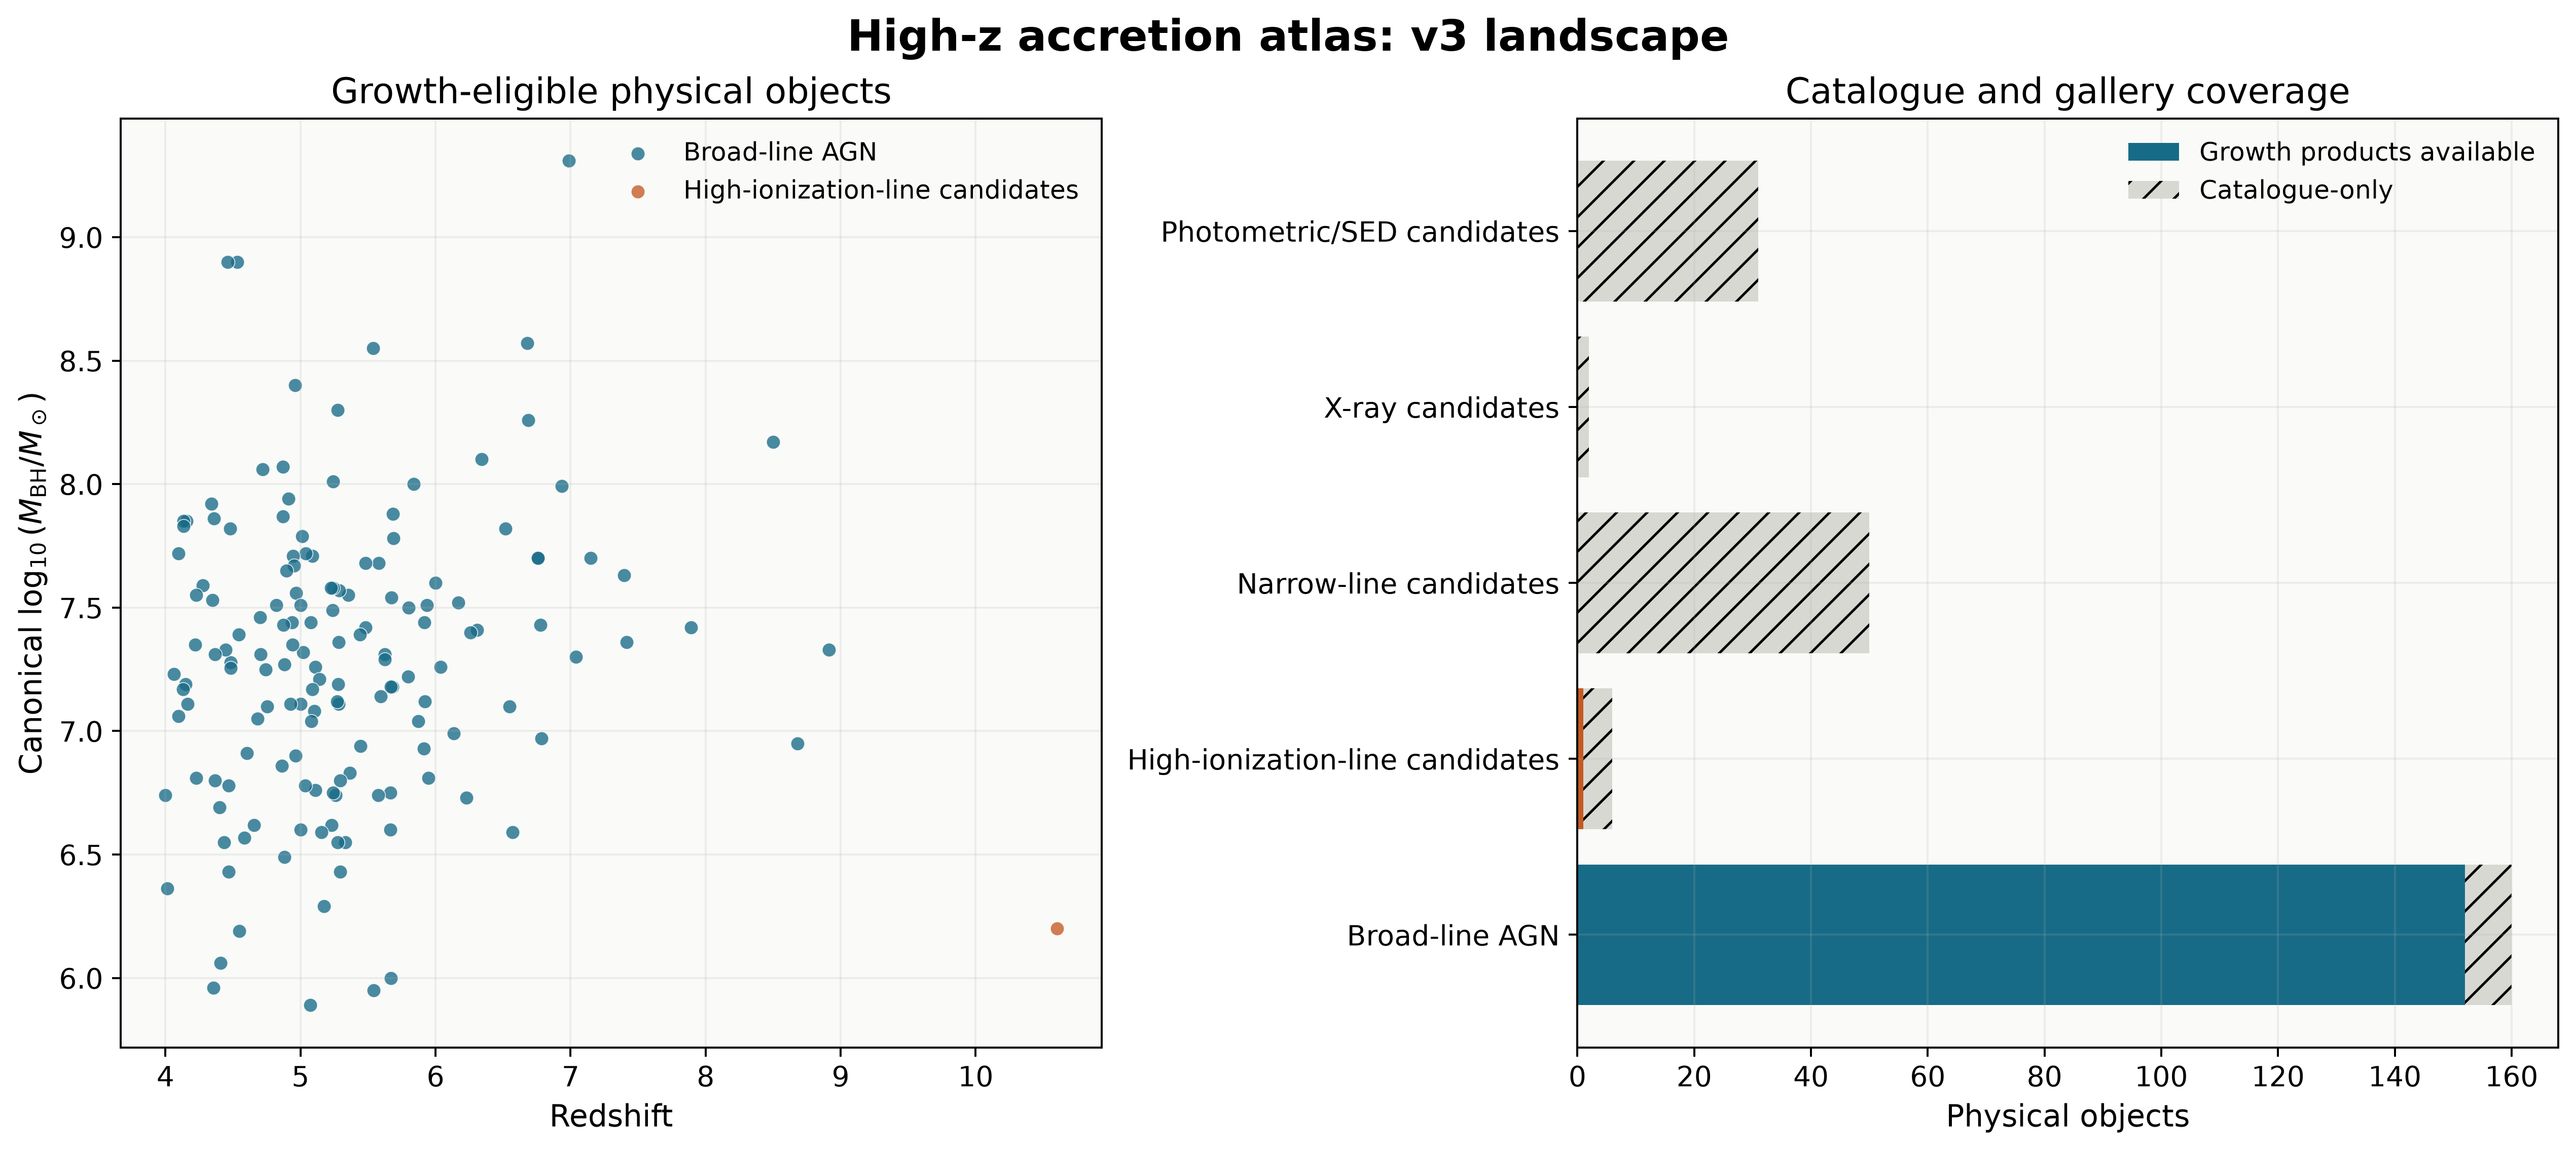
\includegraphics[width=0.99\textwidth]{../results/v3/figures/v3_catalogue_growth_landscape.png}
\caption{Catalogue landscape. Left: the 237 growth-eligible object records in
black-hole-mass--redshift space. Right: product coverage for all 338 objects.
The 101 catalogue-only objects remain available for provenance and evidence
analysis without unsupported numerical growth products.}
\label{fig:landscape}
\end{figure}

\section{Growth-model comparison}

\subsection{Reference model}

We apply the relations in Section~\ref{sec:theory} to each eligible object.
The reference ranking uses $z_{\rm seed}=30$, $\epsilon=0.1$,
$B_{\rm merge}=1$, and $\mseed=10^2\,M_\odot$. Required average rates and
seed masses follow Eqs.~\ref{eq:required-rate} and \ref{eq:required-seed}.
We call the derived requirement \emph{growth pressure}: it measures how
demanding a specified history is, conditional on the published mass and model.
A single merger factor and fixed efficiency do not resolve feedback cycles,
changing accretion states, or stochastic mergers.

The spin-dependent $\fedd$--seed-mass maps and compatibility matrices use
Eq.~\ref{eq:effective-efficiency}. The baseline rankings, duty-cycle diagnostics,
and seed-redshift--mass maps retain $\epsilon=0.1$; growth tracks retain their
stated constant efficiencies. Thus compatibility above unity is conditional on
a different efficiency model from the baseline required-$\fedd$ ranking.

\subsection{Uncertainty and ranking policy}

Published asymmetric mass uncertainties in $\log_{10}\mbh$ are
propagated with 10,000 deterministic split-side draws per measurement and per
preferred object. If a source gives no reported mass error, the atlas does not
invent one. In particular, the twelve mass-bearing NEXUS objects have no
published mass errors. Their repeated point values yield zero-width
stored intervals; probabilities and uncertainty ranks are left unavailable,
not interpreted as certainty. They are marked separately in uncertainty figures. The other
225 objects have reported mass errors. Split-side sampling assigns half
the probability to each side of the reported central value, using the respective
error as the scale of a half-normal distribution; it approximates quoted
intervals rather than reconstructing source posteriors. Redshifts are held
fixed. Draws use seed 20260808 with a stable identifier-based random stream.
For 10,000 draws the binomial Monte Carlo standard error of an estimated
probability is at most 0.005 (approximately 0.0022 at probability 0.95);
this numerical sampling error is separate from astrophysical uncertainty.
Source-reported errors are retained as quoted and are not assumed to be
purely statistical. For ZS7, the published 0.4-dex error already includes
virial-calibration scatter. No additional scatter is added to that error.
Separately reported method-scale systematics are stored and, where possible,
mapped to sensitivity envelopes; the atlas does not assume that these terms
are independent Gaussian errors.

The final published Killi mass $8^{+0.5}_{-0.4}\times10^8M_\odot$
is converted by transforming both linear bounds, giving
$\log_{10}(M/M_\odot)=8.90309^{+0.02633}_{-0.02228}$.

The primary scientific comparison is within object class and mass-comparability
group. Global point and uncertainty ranks are retained only for navigation.
The required-$\fedd$ comparisons in this manuscript use the physical growth
requirement directly. The separate heuristic navigation score and tie policy
are specified in Appendix~\ref{app:navigation}; they do not define the
scientific conclusions.
Compatibility is also calculated object by object across four seed families,
three spin/efficiency cases, two merger cases, and three average accretion rates.
For fixed $z_{\rm seed}=30$, $\epsilon$, $B_{\rm merge}$ and $\fedd$, a cell is
compatible precisely when the required $\log_{10}(M_{\rm seed}/M_\odot)$ lies
inside the inclusive seed interval: $[1,2]$ (light), $[3,4]$ (intermediate),
$[4,6]$ (heavy), or $[2,6]$ (PBH-labelled). These are overlapping scenario
ranges, not probability priors. A required seed below the interval indicates
that this fixed history would overgrow the observed mass; it does not exclude
the seed family under a shorter duty cycle. The PBH label specifies only a
mass range at the common starting redshift, not primordial formation physics
or a PBH abundance constraint.
The source-level selection registry leaves inverse-probability weights unset
because no common inclusion-probability model spans the 32 source families.
Consequently, compatibility fractions are descriptive summaries of the admitted
objects, not population frequencies.

\begin{figure}[p]
\centering
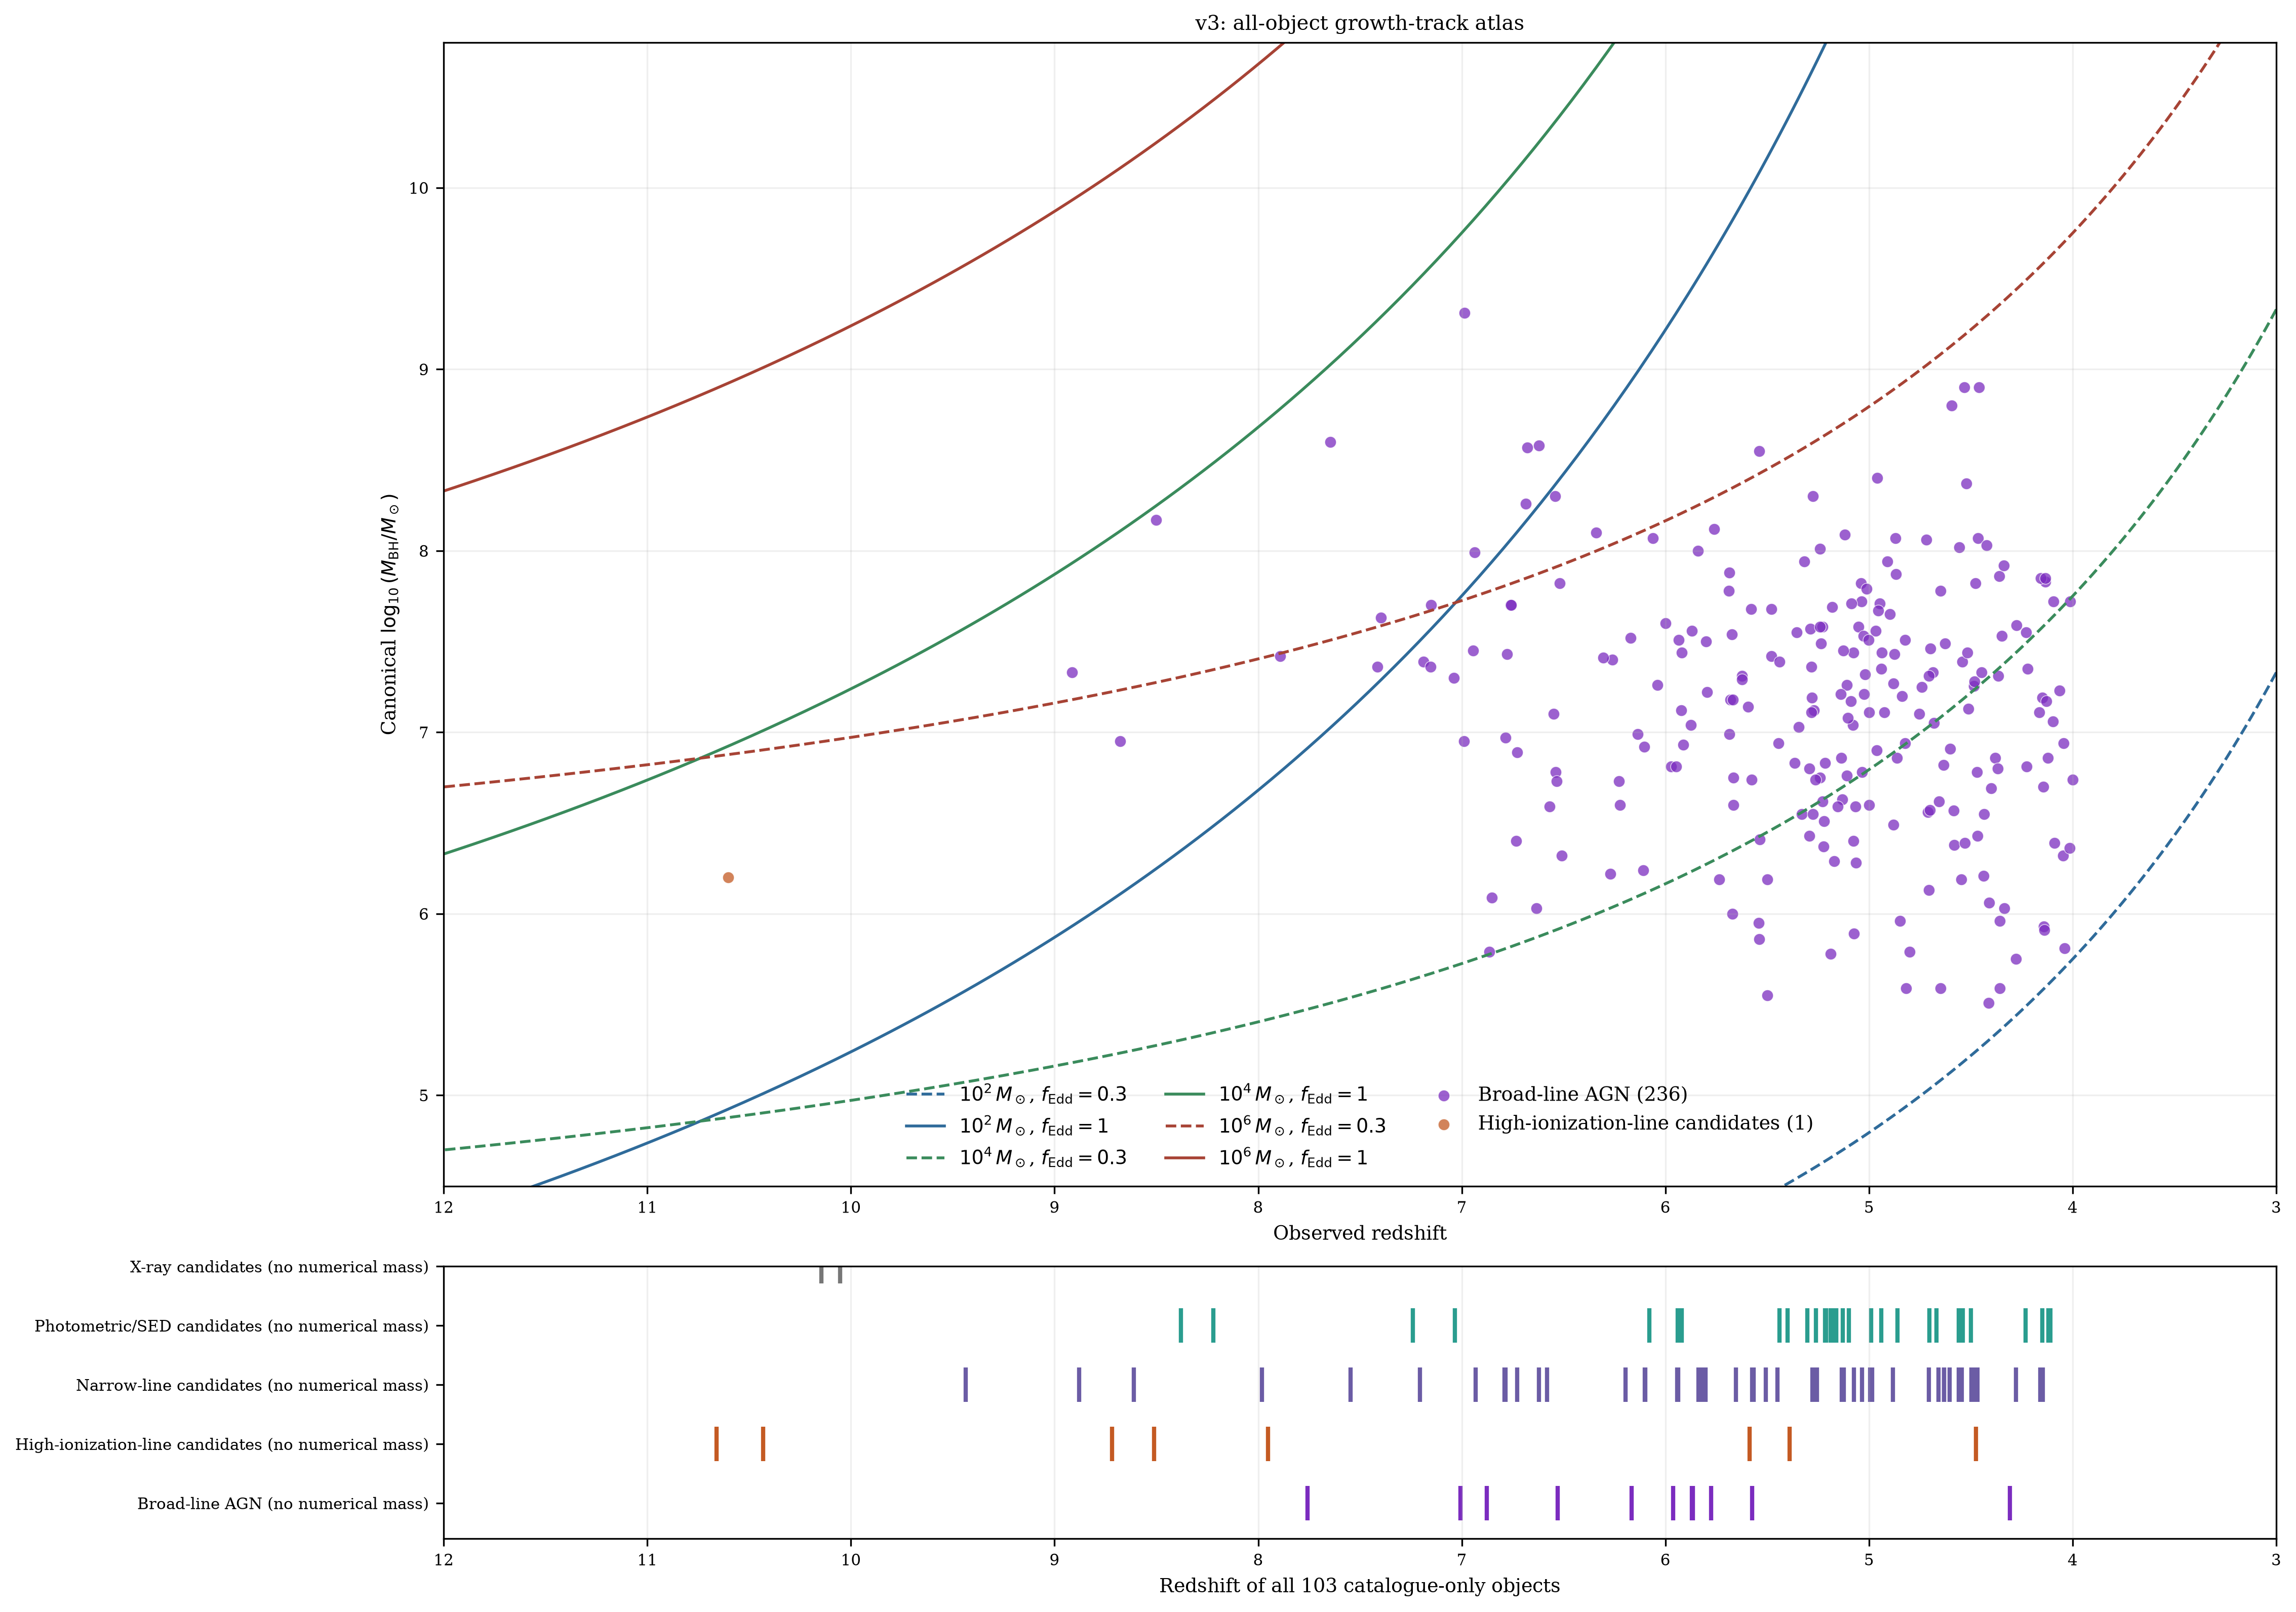
\includegraphics[width=0.99\textwidth]{../results/v3/figures/v3_all_object_growth_tracks.png}
\caption{All-object growth-track view. The upper panel compares the 237
supported masses with reference tracks; the lower panel retains the redshift and
class of all 101 no-mass objects. The reversed redshift axis spans $z=13$ to
$z=3$.}
\label{fig:allgrowth}
\end{figure}

\section{Results}

\subsection{Growth pressure under the reference assumptions}

In the 227-object primary sample, the required $\fedd$ distribution for a
$10^2\,M_\odot$ seed has median 0.574 and interquartile range 0.487--0.684.
Twelve objects require $\fedd>1$ at their point estimates; none requires
$\fedd>2$. The exploratory 237-object sample has median 0.574,
interquartile range 0.488--0.680, and 14 point requirements above unity. The high-pressure
tail is not simply a mass ranking because less cosmic time can offset a lower
observed mass. GN-z11, for example, has a lower standardized mass than many
broad-line objects but has the second-largest required $\fedd$ at
$z=10.603$. Its UV virial estimator and high-ionization evidence place it
outside the primary comparison subset; this position is a conditional
cross-method diagnostic, not a claim of equivalent mass-estimator reliability.

UNCOVER-20466 has the largest required average rate in both samples. Its
point-estimate required $\fedd$ is 1.452, and its Monte Carlo median is 1.453
with a 16th--84th percentile interval of 1.354--1.549.
Table~\ref{tab:top} reports the five largest primary-sample point requirements.
GN-z11 is discussed separately as an exploratory cross-method comparison.

\begin{table}[ht]
\centering
\caption{Highest point-estimate required $\fedd$ for a $10^2\,M_\odot$ seed under
the reference assumptions. Intervals propagate published mass
errors only. All five objects belong to the 227-object primary subset;
GN-z11 is excluded from this comparison.}
\begin{tabular}{@{}lrrrr@{}}
\toprule
Object & $z$ & $\log_{10}(\mbh/M_\odot)$ & Required $\fedd$ & 16th--84th percentile \\
\midrule
UNCOVER-20466 & 8.500 & 8.17 & 1.452 & 1.354--1.549 \\
GS-20057765 & 8.913 & 7.33 & 1.355 & 1.177--1.513 \\
COSMOS3D-13852 & 7.646 & 8.60 & 1.314 & 1.247--1.384 \\
RUBIES-EGS-55604 & 6.986 & 9.31 & 1.267 & 1.250--1.284 \\
CEERS-1019 & 8.679 & 6.95 & 1.205 & 1.115--1.293 \\
\bottomrule
\end{tabular}
\label{tab:top}
\end{table}

\subsection{Robustness to reported mass uncertainty}

Within the primary sample, eight objects remain above unity at the 16th
percentile and six have $P(\fedd>1)\geq0.95$, compared with 12 above unity
at their point estimates. In the exploratory sample, 14 objects have median
required $\fedd>1$, ten remain above unity at the 16th percentile, and 15
cross unity by the 84th percentile; eight have $P(\fedd>1)\geq0.95$. These probabilities are conditional on the
source-reported errors and the reference growth assumptions; they do not add a
common virial-calibration uncertainty or uncertainty in seed redshift,
radiative efficiency, and merger history. These are descriptive counts
within the stated subsets, not population fractions.

\begin{figure}[p]
\centering
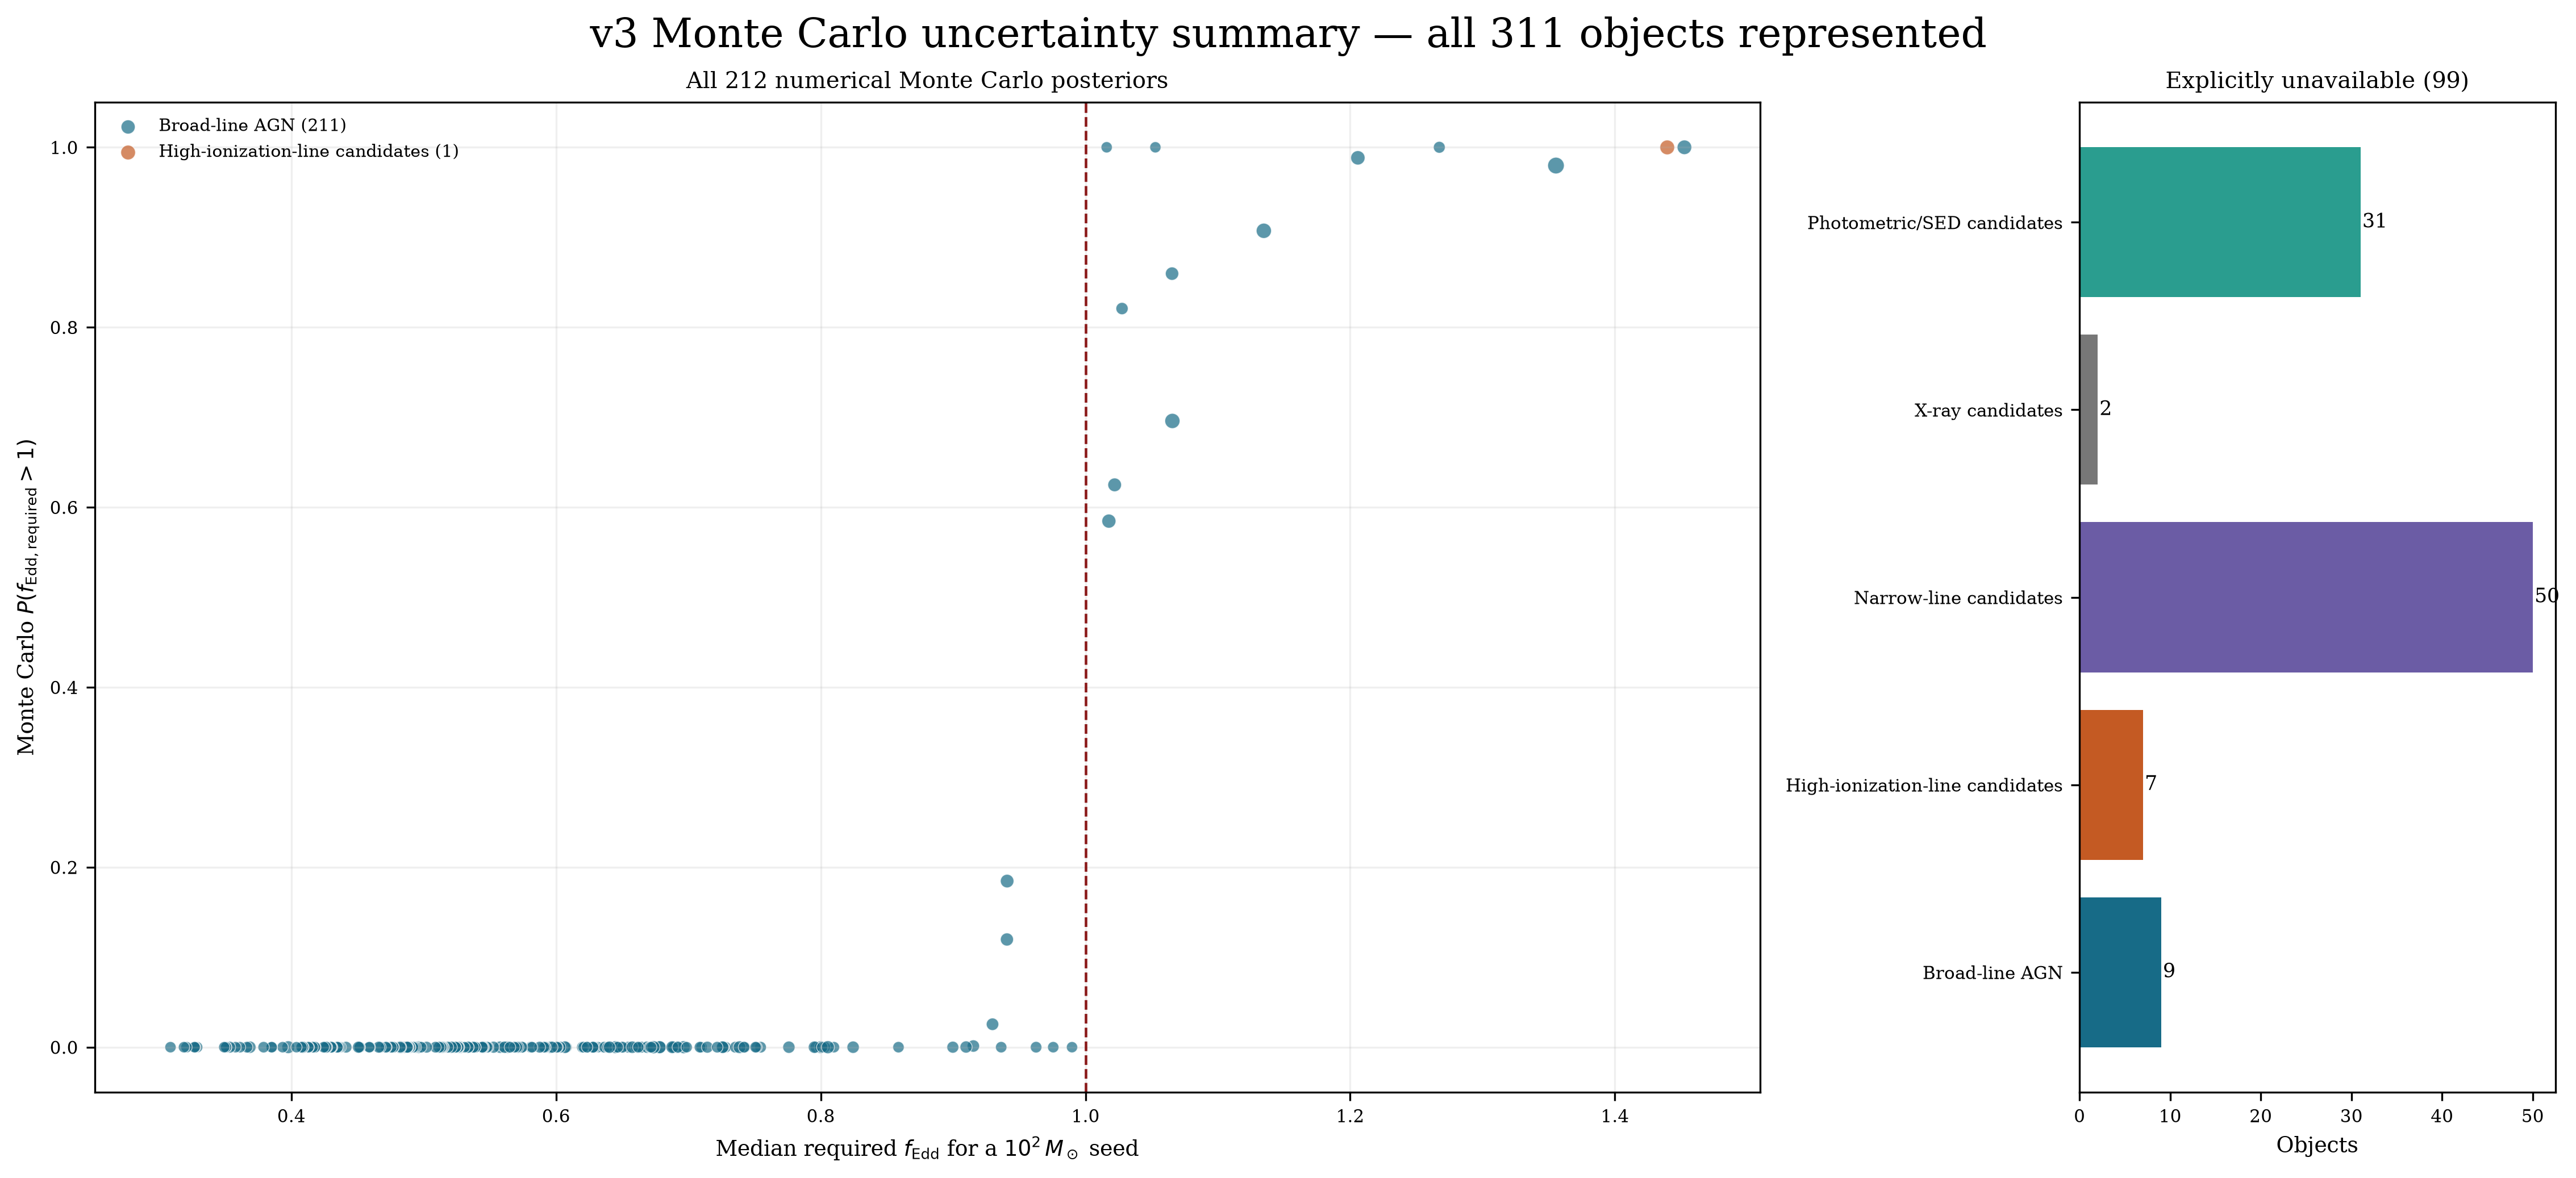
\includegraphics[width=0.99\textwidth]{../results/v3/figures/v3_monte_carlo_summary.png}
\caption{Uncertainty summary for 225 objects with reported mass errors
and 12 point estimates without mass errors, shown as open diamonds on the
``No error'' row. Point size encodes the 16th--84th percentile width for sampled
objects. The accounting panel retains all
101 catalogue-only objects.}
\label{fig:uncertainty}
\end{figure}

A separate publication-version check replaces the frozen Baccus v1
measurements for 44 exact-ID, position-confirmed counterparts with the
published Table~1 values. Five frozen objects lack a published-table
counterpart. Both retaining and omitting those five objects preserve the
headline uncertainty counts above and the top five by required $\fedd$.
The 32 changed central masses shift by $-0.10$ to $+0.04$ dex. This is a
measurement-version sensitivity test with fixed evidence/method taxonomy;
it does not constitute a new admission of the complete published sample.
The object-level comparison and three-scenario summary are distributed
with the v3 science tables.

\subsection{Model compatibility and measurement choice}

Table~\ref{tab:scenarios} isolates changes to the reference history using the
same preferred masses. Increasing the seed mass from $10^2$ to $10^3\,M_\odot$
reduces the primary count above unity from 12 to four; a $10^5\,M_\odot$ seed
removes all point requirements above unity. Delaying seed formation from
$z=30$ to $z=20$ instead raises that count to 22. Lowering the efficiency to
0.05719 removes all point requirements above unity in both samples.
These calculations change one assumption at a time; they are sensitivity
benchmarks, not a joint distribution of physically realized histories.
The seed endpoints bracket the light/heavy alternatives considered in analytic
work \cite{dayal2024}; $10^3\,M_\odot$ probes the transition between them.
The $z=20$ case tests a shorter available growth interval, and the lower
efficiency is the ideal non-spinning thin-disk limit from Eq.~\ref{eq:spin}.
None of these choices is assigned a population weight or inferred from the data.

\begin{table}[ht]
\centering
\caption{Point-estimate requirements above $\overline{\fedd}=1$ under fixed
histories. Each row changes only the named parameter from the reference
($M_{\rm seed}=10^2M_\odot$, $z_{\rm seed}=30$, $\epsilon=0.1$,
$B_{\rm merge}=1$). Counts use provisional object identities and do not include
uncertainty tails.}
\begin{tabular}{@{}lrr@{}}
\toprule
Scenario & Primary (227) & Exploratory (237) \\
\midrule
Reference & 12 & 14 \\
$M_{\rm seed}=10^3M_\odot$ & 4 & 5 \\
$M_{\rm seed}=10^5M_\odot$ & 0 & 0 \\
$z_{\rm seed}=20$ & 22 & 24 \\
$\epsilon=1-\sqrt{8/9}$ & 0 & 0 \\
\bottomrule
\end{tabular}
\label{tab:scenarios}
\end{table}

Compatibility changes substantially across the seed, efficiency, merger, and
average-accretion grid. This dependence is the scientific point of the
compatibility layer: an object's apparent tension cannot be assigned to seed
mass alone without specifying the other assumptions. The complete matrix keeps
unavailable cases distinct from incompatibility, preventing the 101 objects without eligible masses from being counted as failed growth histories.

Seven eligible objects have retained alternate measurements. Their sensitivity
table reports how preferred-measurement choice changes standardized mass and
required $\fedd$. The follow-up matrix separates reference high-pressure objects,
measurement-sensitive cases, and records requiring a suitable mass. Its
categories guide inspection, not model-independent significance or expected
information gain.

\begin{figure}[p]
\centering
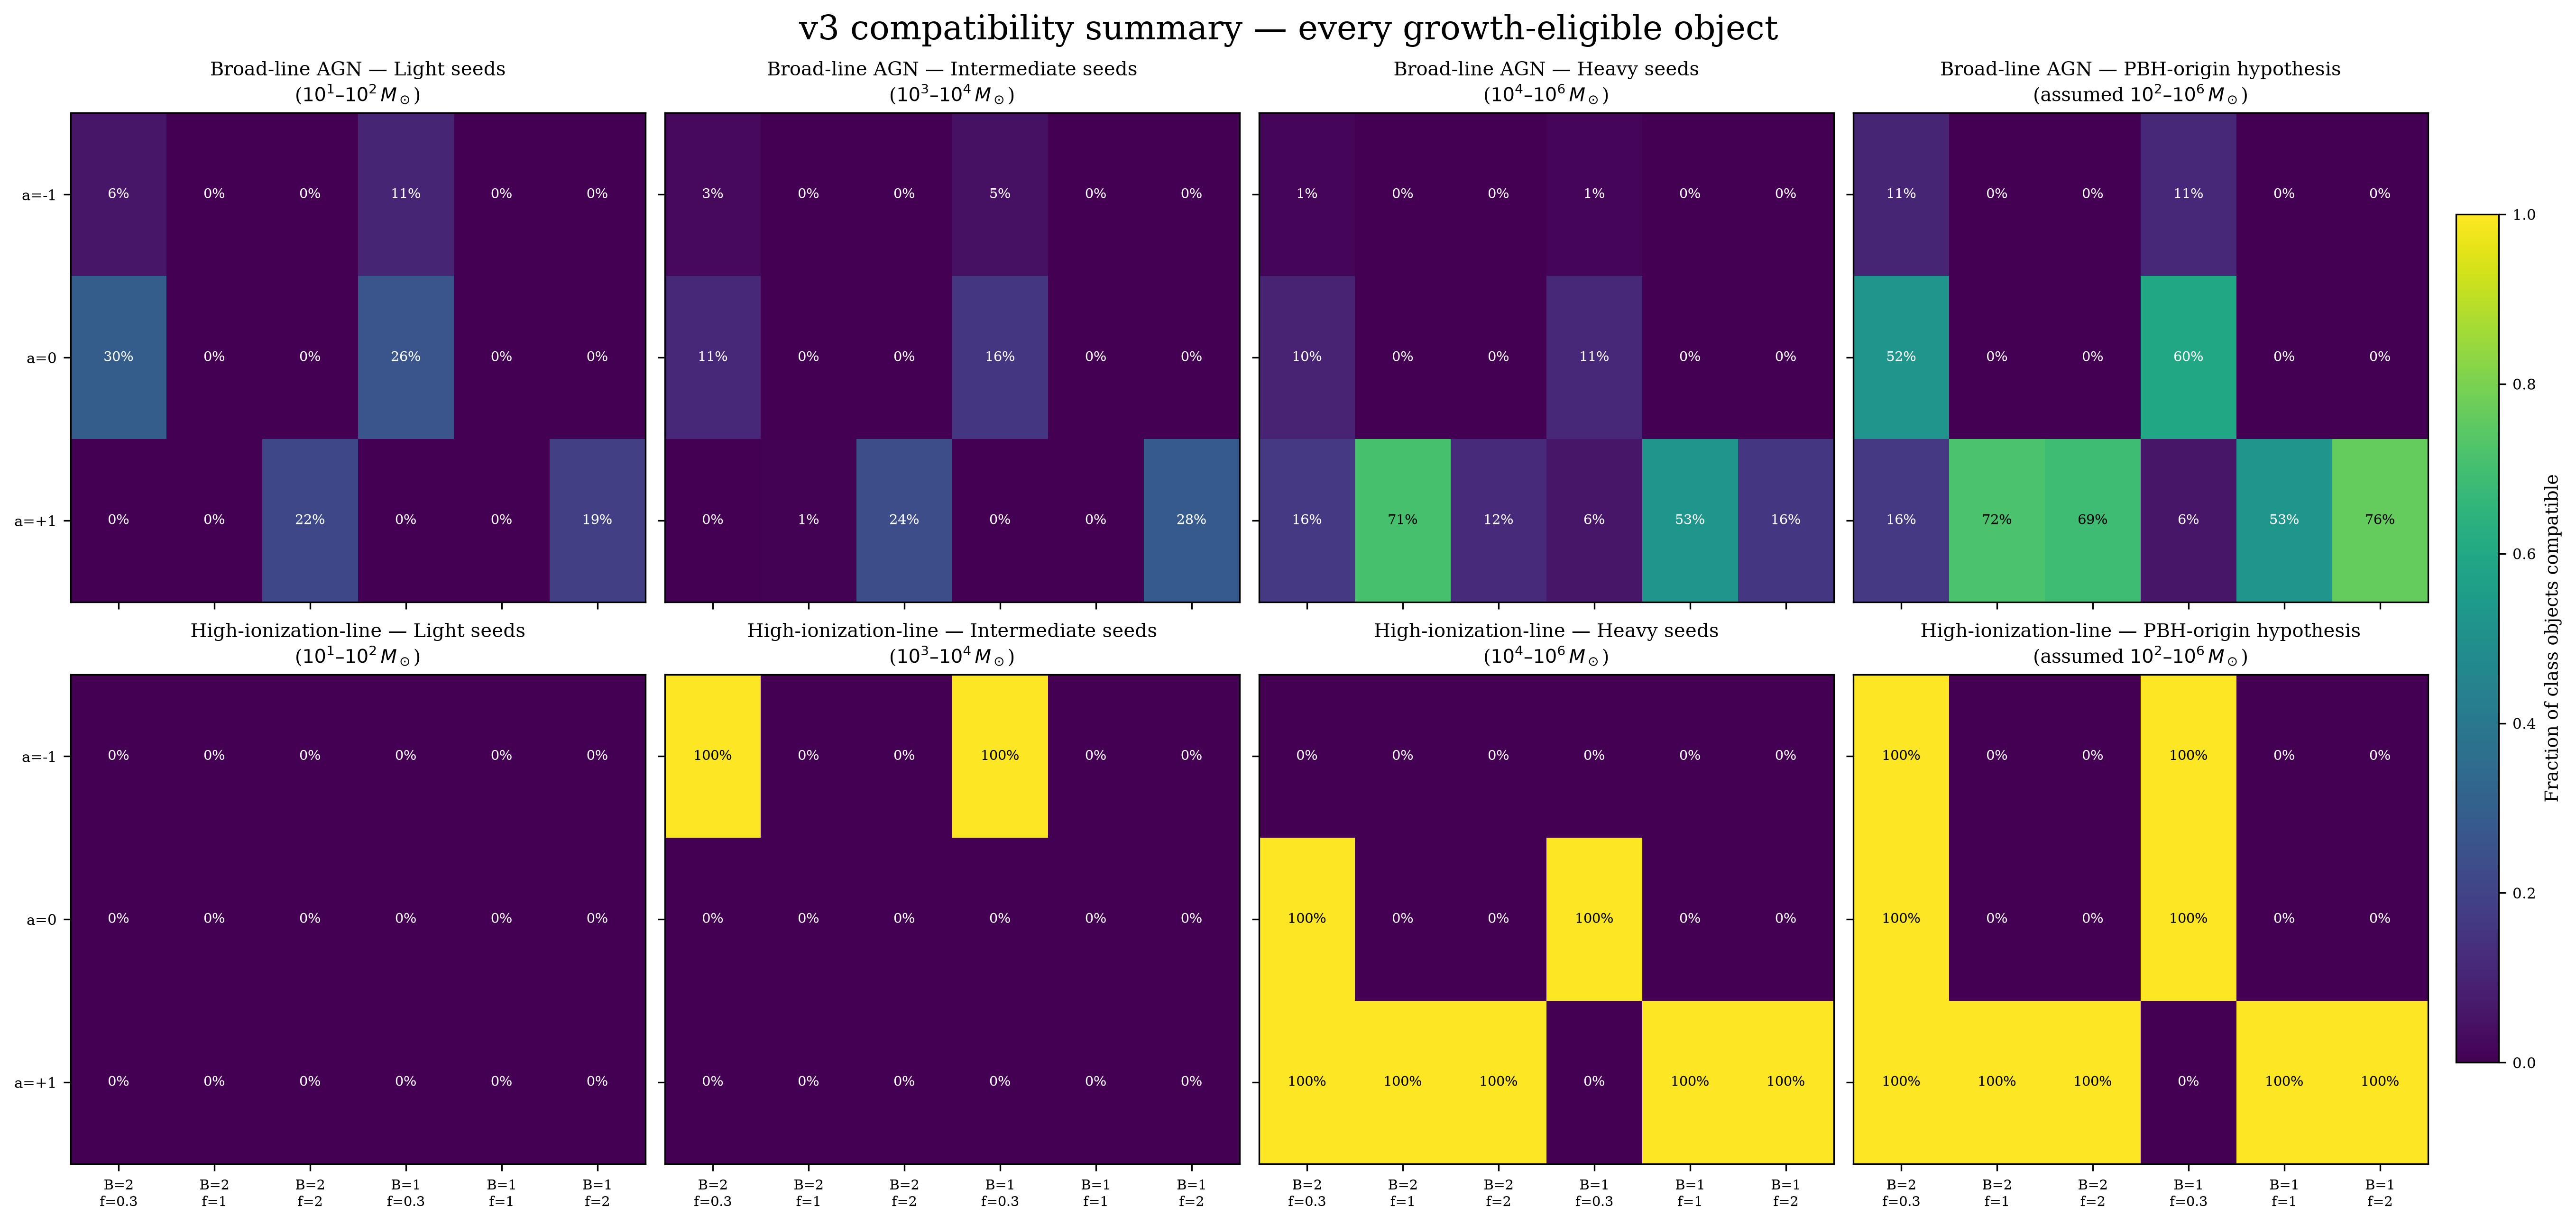
\includegraphics[width=0.99\textwidth]{../results/v3/figures/v3_compatibility_summary.png}
\caption{Descriptive compatibility across seed families, spin/efficiency cases,
merger boosts, and average accretion rates. Percentages are within admitted
classes and are not completeness-corrected demographic estimates.}
\label{fig:compatibility}
\end{figure}

\begin{figure}[p]
\centering
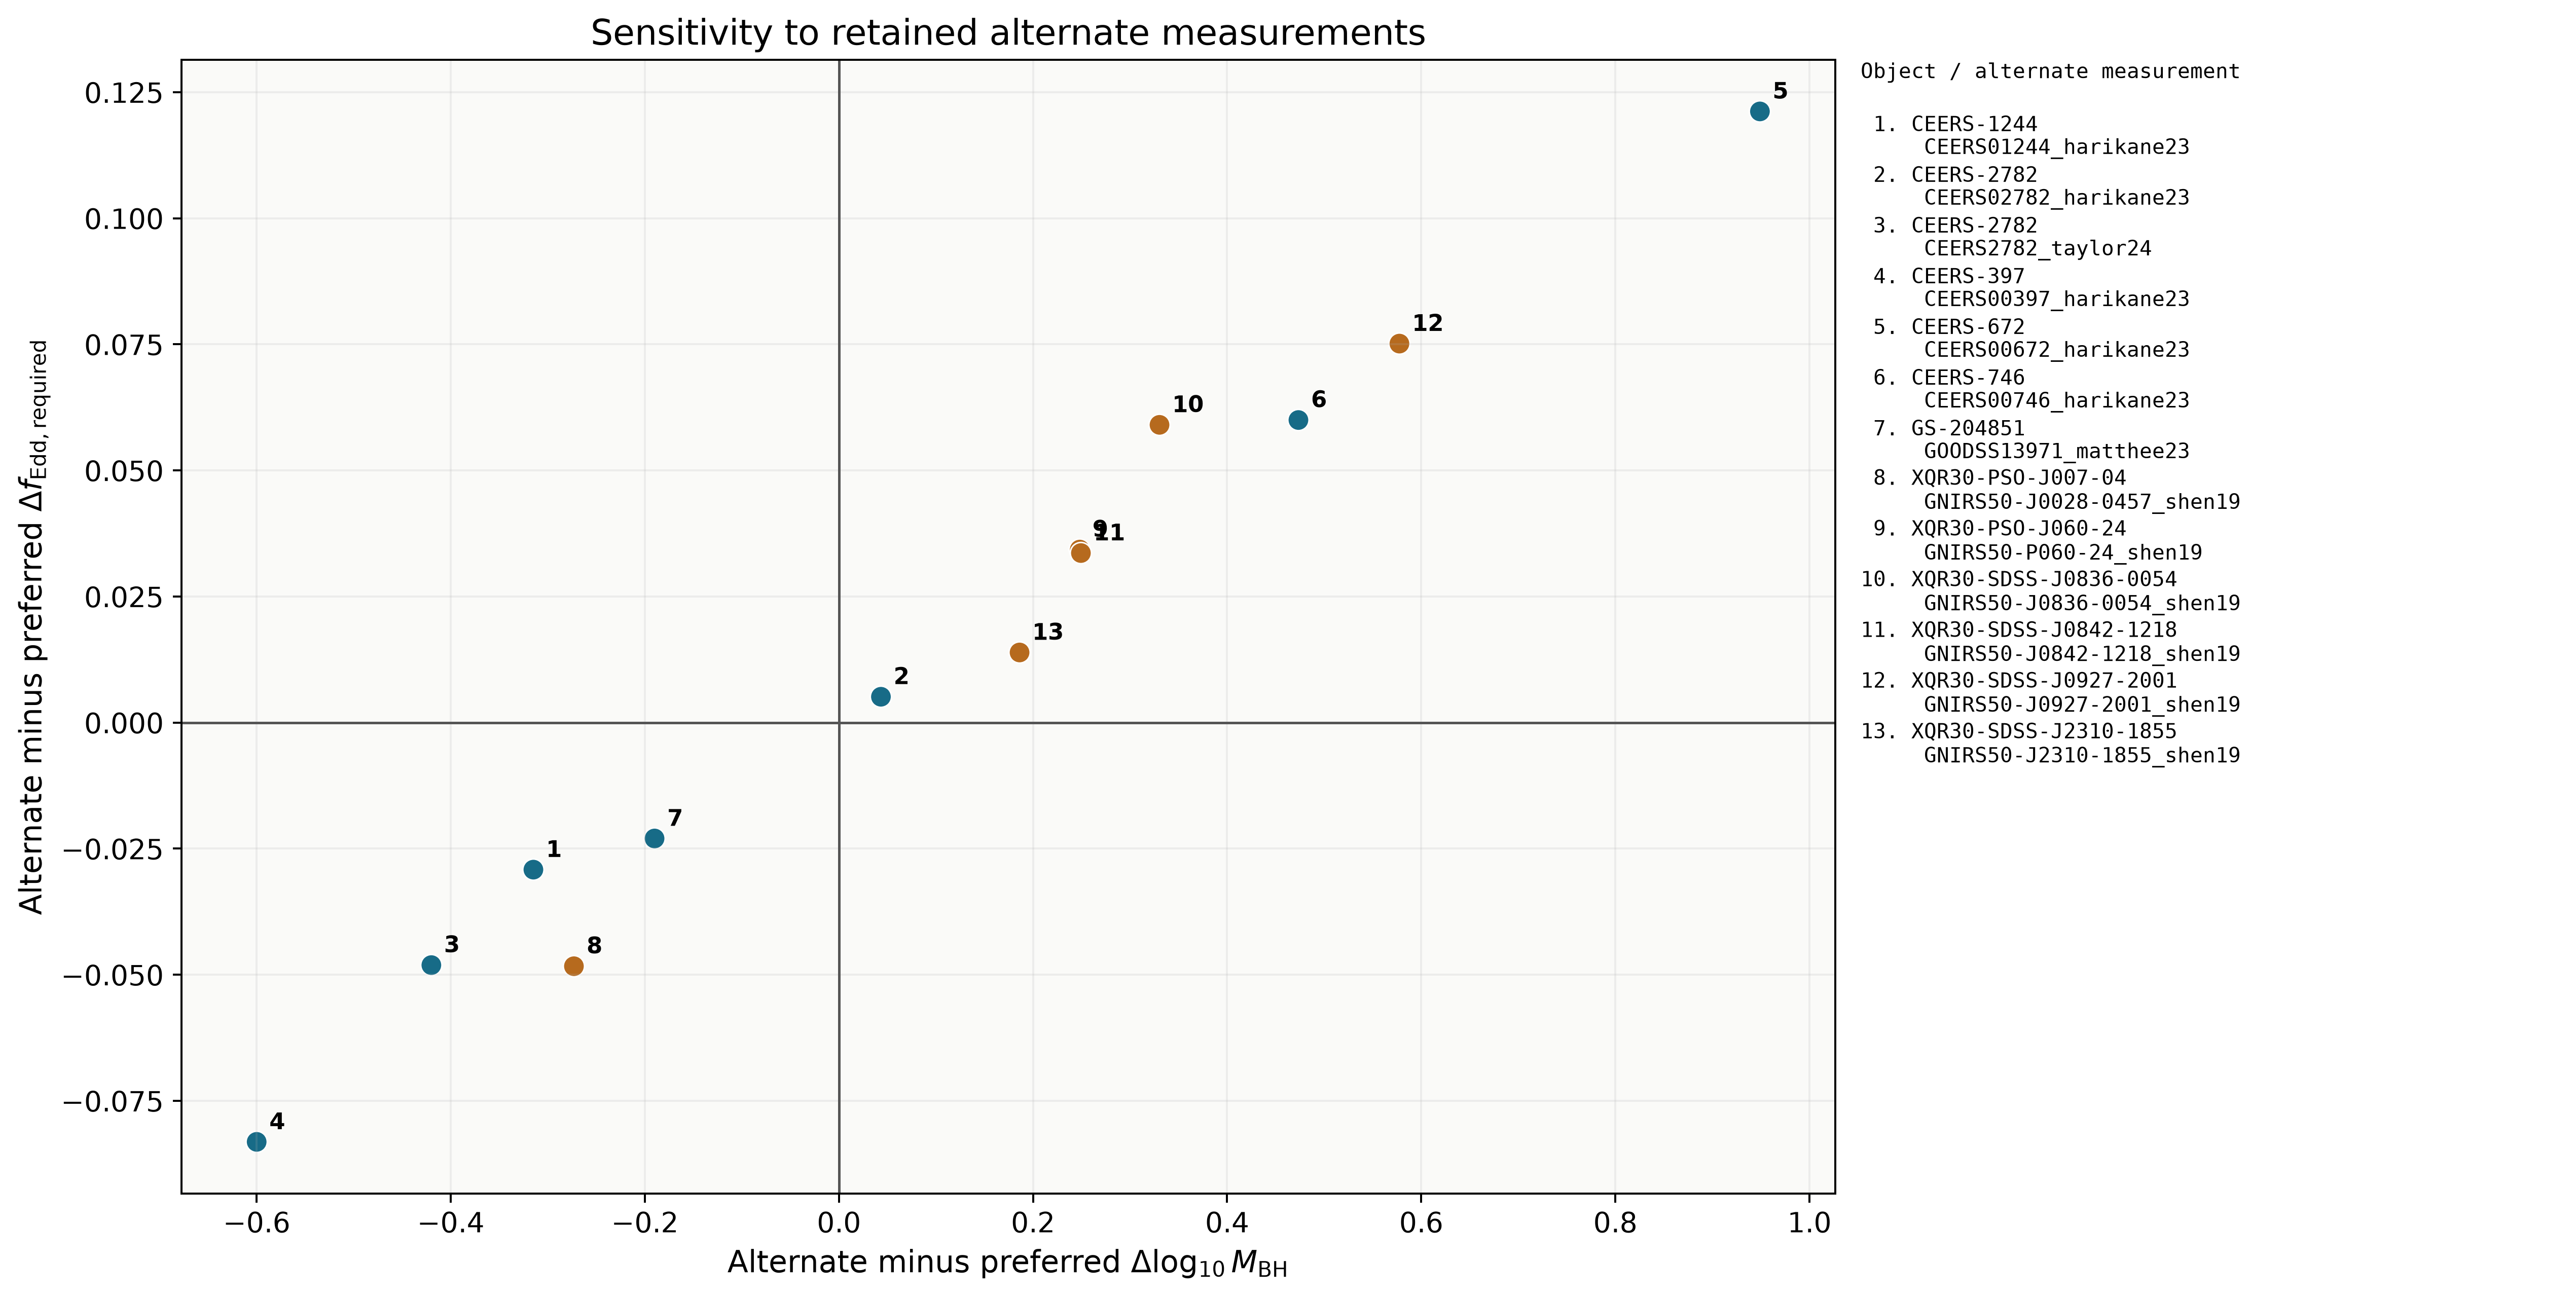
\includegraphics[width=0.99\textwidth]{../results/v3/figures/v3_measurement_sensitivity.png}
\caption{Sensitivity to seven retained alternate measurements. Numbered points
are keyed to stable object and measurement identifiers.}
\label{fig:sensitivity}
\end{figure}
\clearpage

\section{Discussion}

\subsection{What the high-pressure tail establishes}

The scientific question is which objects constrain growth histories and which
constraints survive changes in the assumptions. The 12 primary and 14
exploratory reference point-estimate requirements above unity lie within $z=6.6214$--10.603. The main growth tension is
therefore concentrated in the early subset, not shared by every catalogue
member. The primary 227-object comparison has 12 such requirements; the full
237-object set provides exploratory context across less comparable evidence.


The reference calculation identifies a small set of objects that are difficult
to grow from $10^2\,M_\odot$ seeds at $\fedd\leq1$ under the
reference $\epsilon=0.1$, $z_{\rm seed}=30$ history. The
result does not select a unique remedy. Earlier or heavier seeds, lower effective
radiative efficiency, merger growth, or episodes above the reference accretion
rate can each reduce the tension. The atlas is designed to expose these
trade-offs for each object rather than collapse them into a single formation
label.

This dependence can be quantified without changing the catalogue. At fixed
seed mass, growth interval and merger factor, required $\fedd$ scales as
$\epsilon/(1-\epsilon)$. The implemented ideal non-spinning thin-disk value
$\epsilon=1-\sqrt{8/9}=0.05719$ reduces every point requirement by a factor
0.54594 relative to $\epsilon=0.1$: the largest becomes 0.793 and none exceeds
unity. This sensitivity calculation does not infer actual spins or growth
histories; it shows why the reference tail cannot establish a model-independent
need for super-Eddington accretion.

The efficiency scaling itself is an algebraic consequence of the adopted
model, not a new physical mechanism. The contribution is its application to a
source-traceable catalogue, the assessment of measurement and model sensitivity,
and the identification of objects for which independent observations can most
change the constraints. A point requirement below unity does not exclude
super-Eddington episodes, measure spin, or guarantee a sustainable fuel supply:
near-continuous accretion can remain demanding even when the average is below
Eddington. Scenario compatibility must not be interpreted as a unique history.

The most useful targets are therefore those whose placement is both demanding
and stable to published mass uncertainty. Independent mass measurements,
better separation of broad-line-region kinematics from scattering or outflows,
and constraints on obscuration and lensing can change the physical
interpretation more than another evaluation of the same analytic formula. The
follow-up matrix makes that distinction explicit, but its heuristic ordering is
not a calibrated calculation of expected information gain.

\subsection{Contrasting object-level constraints}

UNCOVER-20466 and GS-20057765 illustrate strong primary-sample constraints on
the reference history: their required averages are 1.452 and 1.355,
respectively, with reported-error 16th percentiles above unity. Increasing the
seed to $10^3M_\odot$ leaves their point requirements above unity (1.217 and
1.101), whereas $10^5M_\odot$ seeds reduce them to 0.746 and 0.592. At the
lower efficiency of 0.05719, the corresponding light-seed requirements are
0.793 and 0.740. Their masses constrain combinations of seed mass and
sustained growth; neither object uniquely selects a seeding channel.
For a quiet state with zero accretion and an Eddington-limited active state,
these latter averages would require active fractions of about 79 and 74 per
cent over the entire available interval. Falling below unity therefore need
not imply an easily sustained fuel supply.

GN-z11 illustrates a different kind of constraint. Its high redshift yields
a reference point requirement of 1.437 despite its smaller adopted mass.
Delaying seeding to $z=20$ raises that requirement to 1.880, exceeding
UNCOVER-20466's 1.733 in that scenario. Thus even the identity of the most
demanding object depends on the starting time. GN-z11's UV estimator and
evidence classification exclude it from the primary sample; an independent,
method-comparable mass would determine whether this apparent timing constraint
survives the measurement assumptions. These examples distinguish sensitivity
to the available growth time from sensitivity to mass methodology.

\subsection{Value of the heterogeneous evidence layer}

The 101 objects without eligible masses remain within project scope because the catalogue is a
cross-paper evidence atlas as well as a growth calculator. Narrow-line,
high-ionization, X-ray, and SED-selected candidates trace discovery channels that
a mass-only broad-line catalogue would omit. They can be compared in redshift,
evidence, survey, and follow-up need, but they are excluded from numerical growth
claims until a suitable mass exists. This separation lets the atlas retain
potentially important early accretors without converting qualitative evidence or
model-dependent context into artificial precision.

\subsection{Limitations}
\label{sec:limits}

The dominant limitations are scientific rather than computational. The
catalogue is a union of heterogeneous selections and cannot support pooled
demographics without source-specific completeness models. Single-epoch virial
masses share calibration and geometry uncertainties that are incompletely
reported across papers. Two source-supported duplicate pairs have been reconciled without removing
measurements. Three identity groups remain open: Baccus GDS\_1210\_9515 versus
JADES GS-8083, GS-10013704 versus Scholtz 99671, and Scholtz 16745 versus 208643.
The first requires target/spectral and preferred-mass reconciliation; the latter
two require imaging and aperture checks. Unique-object and host counts remain
provisional. These specific tasks cannot be replaced by wider matching thresholds. Finally, Eq.~\ref{eq:growth}
compresses time-dependent accretion, feedback, mergers, and radiative-state
changes into effective parameters. Its outputs should be read as conditional
comparisons, not reconstructed histories. Reported-error probabilities condition
on fixed growth parameters; marginalization requires justified parameter
distributions and correlations, not just scenario maps. They are not seed-origin
probabilities. The age relation neglects radiation; the supplementary $z_{\rm seed}=3400$
plot is an extrapolation, not evidence for primordial formation or a physical
radiation-era accretion history.

All admitted numerical mass/error fields have independent source checks;
all 350 central redshifts and 323 available coordinate pairs are also checked
against independent source evidence. Twenty-seven measurement rows lack
coordinates. Redshift uncertainties, full source posteriors, and auxiliary
observables are not exhaustively validated. The immediate priority is resolving
the three identity groups and reassessing affected summaries. The literature
cutoff is 3 September 2026; catalogue completeness refers to the declared source
membership, not every JWST discovery.
Demographic inference requires source-specific inclusion models and overlap
corrections. The A2744-QSO1 direct-mass measurement \cite{juodzbalis_direct2025} awaits a new
dataset version under the frozen-membership policy.

\section{Reproducibility and data products}

The repository provides pinned direct Python dependencies, five ordered
notebooks, versioned catalogues, and hash manifests. Reproduction checks compare
regenerated numerical tables and figures against committed baselines with
explicit numerical and raster tolerances. Independent quadrature of the cosmic
age integral and Runge--Kutta growth integration supplement these comparisons.
The release includes per-object parameter maps, alternate-measurement checks,
and source-linked follow-up information; implementation details and artifact
inventories are documented in the repository.

Independent source checks cover all 244 numerical mass measurements and their
error fields, all 350 central redshifts, and 323 available coordinate pairs.
These establish source-value agreement within the declared checks, not the
physical validity of every mass estimator or the uniqueness of every target.
The separate publication identity gate remains open for the three groups in
Section~\ref{sec:limits}. A successful computational reproduction does not
close that scientific gate.

\section{Conclusions}

We have constructed a reproducible atlas with 338 provisional object records of JWST-identified accreting
black-hole objects and candidates at $z\geq4$. The main results are:
\begin{itemize}
\item 237 objects have a numerically eligible mass and 101 remain explicit
no-inference records;
\item in the primary 227-object sample, the light-seed reference history gives
12 point requirements above $\fedd=1$, eight above unity at the 16th percentile,
and six with $P(\fedd>1)\geq0.95$; the exploratory counts are 14, ten, and eight;
\item increasing the seed mass to $10^3M_\odot$ reduces the primary point count
to four, while delaying seeding to $z=20$ increases it to 22; object ordering
also depends on the assumed starting time;
\item model compatibility is conditional on seed, efficiency, merger, and
accretion assumptions, and the heterogeneous catalogue cannot support pooled
demographic inference; lowering the fixed efficiency to the ideal non-spinning
value removes all point-estimate requirements above unity; and
\item complete provenance, identity history, uncertainty semantics, source
caveats, follow-up priorities, and per-object visual products remain linked to
the same frozen v3 dataset.
\end{itemize}

The immediate next step is to resolve the three remaining identity groups and
reassess affected summaries. Within the present object-level scope, independent
mass constraints and physically justified growth scenarios can then identify
which conclusions are stable. Population inference would additionally require
survey completeness, overlap corrections, and shared mass-calibration modelling.

\appendix
\section{Source-family inventory}
\label{app:sources}

The input literature spans JWST broad-line samples
\cite{juodzbalis2026,taylor2025,matthee2024,lin2024,harikane2023,davis2026,
greene2024,kocevski2025,skyfire2026,larson2023,killi2024,ubler2024,
baccus2026,fei2026,zhuang2025,lin2025}, host-selected broad-line candidates
\cite{ren2025}, an X-ray evidence history \cite{bogdan2024,zou2026}, JADES
narrow/high-ionization candidates \cite{scholtz2025}, and GN-z11
high-ionization evidence \cite{maiolino2024}. Heterogeneous additions include
high-ionization and narrow-line candidates
\cite{chisholm2024,tang2025,mazzolari2024,zhang2026,chavezortiz2026}, MIRI
SED-selected candidates \cite{leung2026,lyu2024}, GHZ9
\cite{napolitano2025}, compact blue broad-line emitters \cite{mascia2026},
additional UNCOVER candidates \cite{treiber2025}, MoM-BH*-1
\cite{naidu2026}, and GHZ4/GHZ7 \cite{napolitano2024}.

\section{Catalogue navigation score}
\label{app:navigation}

The point navigation score is
\begin{equation}
S=\min\left[100,100\max\left(C\!\left(\frac{f_2-0.3}{1.2}\right),
C\!\left(\frac{s_{0.3}-4}{2.8}\right)\right)
+8C\!\left(\frac{z-6}{4}\right)\right],
\end{equation}
where $C(x)=\min(1,\max(0,x))$, $f_2$ is the required
$\fedd$ for a $10^2\,M_\odot$ seed, and $s_{0.3}$ is the required
$\log_{10}(M_{\rm seed}/M_\odot)$ at $\fedd=0.3$. This heuristic combines
two growth diagnostics and a redshift term; it is not a probability. Ties use
decreasing $f_2$, decreasing redshift, then stable identifier. The manuscript's
required-$\fedd$ table is instead ordered directly by $f_2$.
\section{Release inventory}

Canonical manifests record SHA-256 hashes for 85 v1, 461 v2, and 720 v3 artifacts.
The current result inventory contains 1,236 artifacts. These inventories have
different scopes: version manifests include dataset products as well as results.
The repository records their individual entries and verification tolerances.

\begin{thebibliography}{99}
\setlength{\itemsep}{2pt}
\bibitem{bardeen1972} Bardeen, J. M., Press, W. H., \& Teukolsky, S. A. 1972,
\emph{ApJ}, 178, 347--369, doi:10.1086/151796.
\bibitem{dayal2024} Dayal, P. 2024, \emph{A\&A}, 690, A182, doi:10.1051/0004-6361/202451481.
\bibitem{juodzbalis2026} Juod\v{z}balis, I. et al. 2026, \emph{MNRAS}, 546, stag086, doi:10.1093/mnras/stag086.
\bibitem{taylor2025} Taylor, A. J. et al. 2025, \emph{ApJ}, 986, 165, doi:10.3847/1538-4357/add15b.
\bibitem{matthee2024} Matthee, J. et al. 2024, \emph{ApJ}, 963, 129, doi:10.3847/1538-4357/ad2345.
\bibitem{lin2024} Lin, X. et al. 2024, \emph{ApJ}, 974, 147, doi:10.3847/1538-4357/ad6565.
\bibitem{harikane2023} Harikane, Y. et al. 2023, \emph{ApJ}, 959, 39, doi:10.3847/1538-4357/ad029e.
\bibitem{davis2026} Davis, K. et al. 2026, arXiv:2602.23310v1.
\bibitem{hutchison2025} Hutchison, T. A. et al. 2025, THRILS redshift catalogue, arXiv:2512.12509v1.
\bibitem{ren2025} Ren, J. et al. 2025, \emph{MNRAS}, 544, 211--233, doi:10.1093/mnras/staf1709.
\bibitem{greene2024} Greene, J. E. et al. 2024, \emph{ApJ}, 964, 39, doi:10.3847/1538-4357/ad1e5f.
\bibitem{kocevski2025} Kocevski, D. D. et al. 2025, \emph{ApJ}, 986, 126, doi:10.3847/1538-4357/adbc7d.
\bibitem{skyfire2026} Skyfire Collaboration 2026, arXiv:2609.00112v1.
\bibitem{larson2023} Larson, R. L. et al. 2023, \emph{ApJL}, 953, L29, doi:10.3847/2041-8213/ace619.
\bibitem{killi2024} Killi, M. et al. 2024, \emph{A\&A}, 691, A52, doi:10.1051/0004-6361/202348857.
\bibitem{ubler2024} \"{U}bler, H. et al. 2024, \emph{MNRAS}, 531, 355, doi:10.1093/mnras/stae943.
\bibitem{baccus2026} Baccus, C. et al. 2026, \emph{ApJ}, 1006, 165, doi:10.3847/1538-4357/ae7de7.
\bibitem{fei2026} Fei, Q. et al. 2026, \emph{ApJ}, 1003, 244, doi:10.3847/1538-4357/ae6248.
\bibitem{bogdan2024} Bogd\'an, \'A. et al. 2024, \emph{Nature Astronomy}, 8, 126, doi:10.1038/s41550-023-02111-9.
\bibitem{goulding2023} Goulding, A. D. et al. 2023, \emph{ApJL}, 955, L24, doi:10.3847/2041-8213/acf7c5.
\bibitem{zou2026} Zou, F. et al. 2026, UHZ1 full-data X-ray reanalysis, accepted by \emph{ApJ}, arXiv:2603.24893v2.
\bibitem{scholtz2025} Scholtz, J. et al. 2025, \emph{A\&A}, 697, A175, doi:10.1051/0004-6361/202348804.
\bibitem{maiolino2024} Maiolino, R. et al. 2024, \emph{Nature}, 627, 59--63, doi:10.1038/s41586-024-07052-5.
\bibitem{chisholm2024} Chisholm, J. et al. 2024, \emph{MNRAS}, doi:10.1093/mnras/stae2199.
\bibitem{tang2025} Tang, M. et al. 2025, accepted by \emph{ApJ}, arXiv:2505.06359v2.
\bibitem{mazzolari2024} Mazzolari, G. et al. 2024, \emph{A\&A}, 691, A338, doi:10.1051/0004-6361/202451860.
\bibitem{leung2026} Leung, G. C. K. et al. 2026, submitted to \emph{ApJ}, arXiv:2607.02666v1.
\bibitem{lyu2024} Lyu, J. et al. 2024, \emph{ApJ}, 966, 229, doi:10.3847/1538-4357/ad3643.
\bibitem{napolitano2025} Napolitano, L. et al. 2025, \emph{ApJ}, 989, 75, doi:10.3847/1538-4357/ade706.
\bibitem{zhang2026} Zhang, Z. et al. 2026, accepted by \emph{ApJ}, arXiv:2506.04350v2.
\bibitem{chavezortiz2026} Chavez Ortiz, O. A. et al. 2025, revised 2026, arXiv:2511.03035v2.
\bibitem{mascia2026} Mascia, S. et al. 2026, submitted to \emph{A\&A}, arXiv:2608.25021v1.
\bibitem{treiber2025} Treiber, H. et al. 2025, \emph{ApJ}, 984, 93, doi:10.3847/1538-4357/adc38f.
\bibitem{naidu2026} Naidu, R. P. et al. 2026, \emph{Nature}, 656, 329--333, doi:10.1038/s41586-026-10846-4.
\bibitem{zhuang2025} Zhuang, M.-Y. et al. 2025, NEXUS broad-line AGN sample, arXiv:2505.20393v1.
\bibitem{lin2025} Lin, X. et al. 2025, COSMOS-3D broad-line AGN sample, accepted by \emph{ApJ}, doi:10.3847/1538-4357/ae1b9b.
\bibitem{napolitano2024} Napolitano, L. et al. 2025, \emph{A\&A}, 693, A50, doi:10.1051/0004-6361/202452090.
\bibitem{juodzbalis_direct2025} Juod\v{z}balis, I. et al. 2025,
A direct black hole mass measurement in a Little Red Dot at the Epoch of
Reionization, arXiv:2508.21748v2; related publication doi:10.1038/s41586-026-10579-4.
\end{thebibliography}

\end{document}
